\documentclass{standalone}
\usepackage[dvipsnames]{xcolor}
\usepackage{tikz}
\usetikzlibrary{positioning, calc, shapes, fit}

\begin{document}

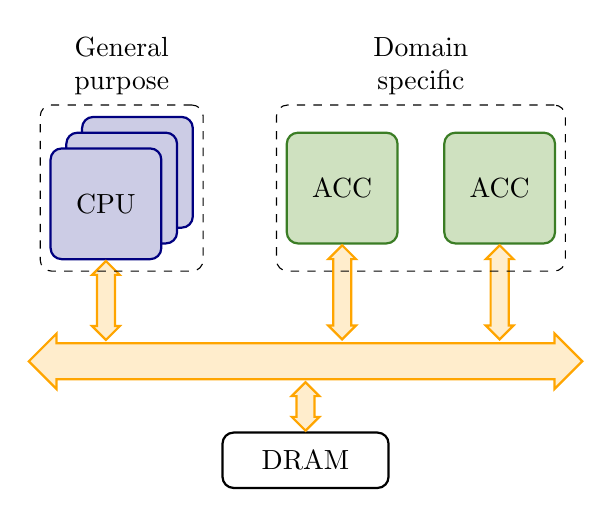
\begin{tikzpicture}
  \tikzstyle{PE}=[rounded corners, draw, thick, minimum size=40pt, align=center]
  \tikzstyle{core}=[PE, draw=NavyBlue, fill=NavyBlue!20]
  \tikzstyle{hwacc}=[PE, draw=OliveGreen, fill=OliveGreen!20]
  \tikzstyle{bus}=[double arrow, draw=Orange, fill=Orange!20, thick,
  minimum width=20pt, double arrow head extend=2pt]

  \node (core2) at (0.4,0.4) [core] {};
  \node (core1) at (0.2,0.2) [core] {};
  \node (core0) at (0,0) [core] {CPU};

  \node (hwacc1) at (3,0.2) [hwacc] {ACC};
  \node (hwacc2) at (5,0.2) [hwacc] {ACC};

  \node (mainbus) at (-1, -2) [bus, anchor=west, minimum height=200pt] {};

  \node (dram) [draw, rounded corners, below= of mainbus, minimum width=60pt,
  minimum height=20pt, yshift=10pt, thick] {DRAM};

  \node at (dram.north) [bus, rotate=-90, anchor=east, scale=0.5, minimum height=35pt] {};

  \node at (core0.south) [bus, rotate=90, anchor=east, scale=0.5, minimum height=57pt] {};
  \node at (hwacc1.south) [bus, rotate=90, anchor=east, scale=0.5, minimum height=68pt] {};
  \node at (hwacc2.south) [bus, rotate=90, anchor=east, scale=0.5, minimum height=68pt] {};

  \node (gpc) [fit=(core0)(core1)(core2), rounded corners,
  dashed, draw, minimum height=60pt, label={[align=center]90:{General\\ purpose}}] {};
  \node (dsc) [fit=(hwacc1)(hwacc2), rounded corners, dashed,
  draw, minimum height=60pt, label={[align=center]90:{Domain\\ specific}}] {};

\end{tikzpicture}

\end{document}